\documentclass[a4paper,10pt]{article} % Default font size and paper size

%{{{ Packages & Includes
%\usepackage{xunicode,xltxtra,url,parskip} % Formatting packages
\usepackage{url,parskip} % Formatting packages
\usepackage{graphicx}
\usepackage{adjustbox}

\usepackage[usenames,dvipsnames]{xcolor} % Required for specifying custom colors

%\usepackage[big]{layaureo} % Margin formatting of the A4 page, an alternative to layaureo can be \usepackage{fullpage}
% To reduce the height of the top margin uncomment: \addtolength{\voffset}{-1.3cm}
\usepackage[left=2cm,right=2cm,top=1.5cm,bottom=1.5cm]{geometry}
\usepackage{hyperref} % Required for adding links	and customizing them
\definecolor{linkcolour}{rgb}{0,0.2,0.6} % Link color
\hypersetup{colorlinks,breaklinks,urlcolor=linkcolour,linkcolor=linkcolour} % Set link colors throughout the document
\usepackage{array}
\newcolumntype{R}[1]{>{\raggedleft\let\newline\\\arraybackslash\hspace{0pt}}m{#1}}
\newcolumntype{L}[1]{>{\raggedright\let\newline\\\arraybackslash\hspace{0pt}}m{#1}}
\newcolumntype{C}[1]{>{\centering\let\newline\\\arraybackslash\hspace{0pt}}m{#1}}

\usepackage{titlesec} % Used to customize the \section command
\titleformat{\section}{\scshape\raggedright}{}{0em}{}[\titlerule] % Text formatting of sections
\titlespacing{\section}{0pt}{3pt}{3pt} % Spacing around sections
%}}}

% Variable Definition
\newcommand\columnWidth{14.7cm}

\begin{document}

\pagestyle{empty} % Removes page numbering

\section{Personal Information}

\begin{table}[ht]
\begin{minipage}{0.77\linewidth}
    \begin{tabular}{L{1.75cm}p{3cm}p{2cm}L{1.4cm}L{1.5cm}}
        Full Name: & \textbf{Carlos Segarra} & & \multicolumn{2}{l}{\textbf{Languages:}} \\
        Birthday: & 09/06/1996 & & Spanish: & Native\\
        Residence: & Barcelona, Spain & & Catalan: & Native \\
        Website: & \href{https://carlossegarra.com}{carlossegarra.com} & & English: & C2\\
        Mail: & \small{carlossegarragonzalez@gmail.com} & & French: & Fluent \\
        Phone: & +34 699 20 89 00 & & German: & A2
    \end{tabular}
\end{minipage}\hfill
\begin{minipage}{0.2\linewidth}
\centering
%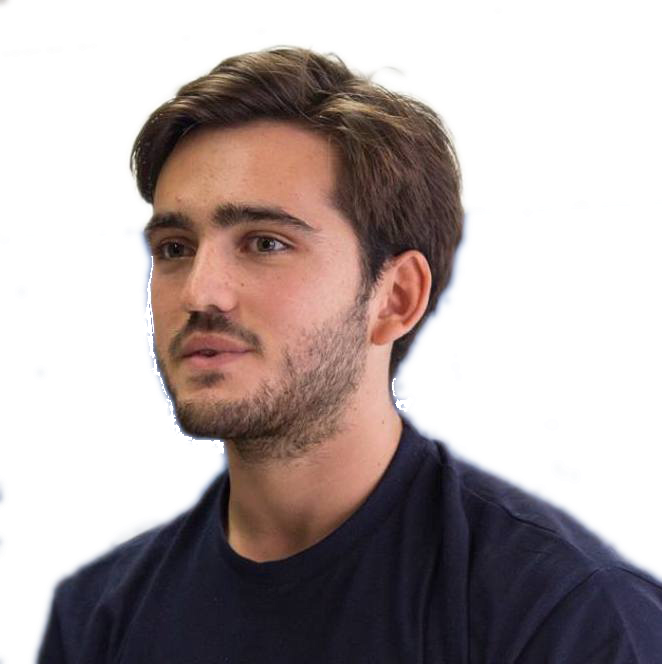
\includegraphics[width=2.5cm]{carlos_portrait.png}
{%
\setlength{\fboxsep}{0pt}%
\setlength{\fboxrule}{0.7pt}%
\fbox{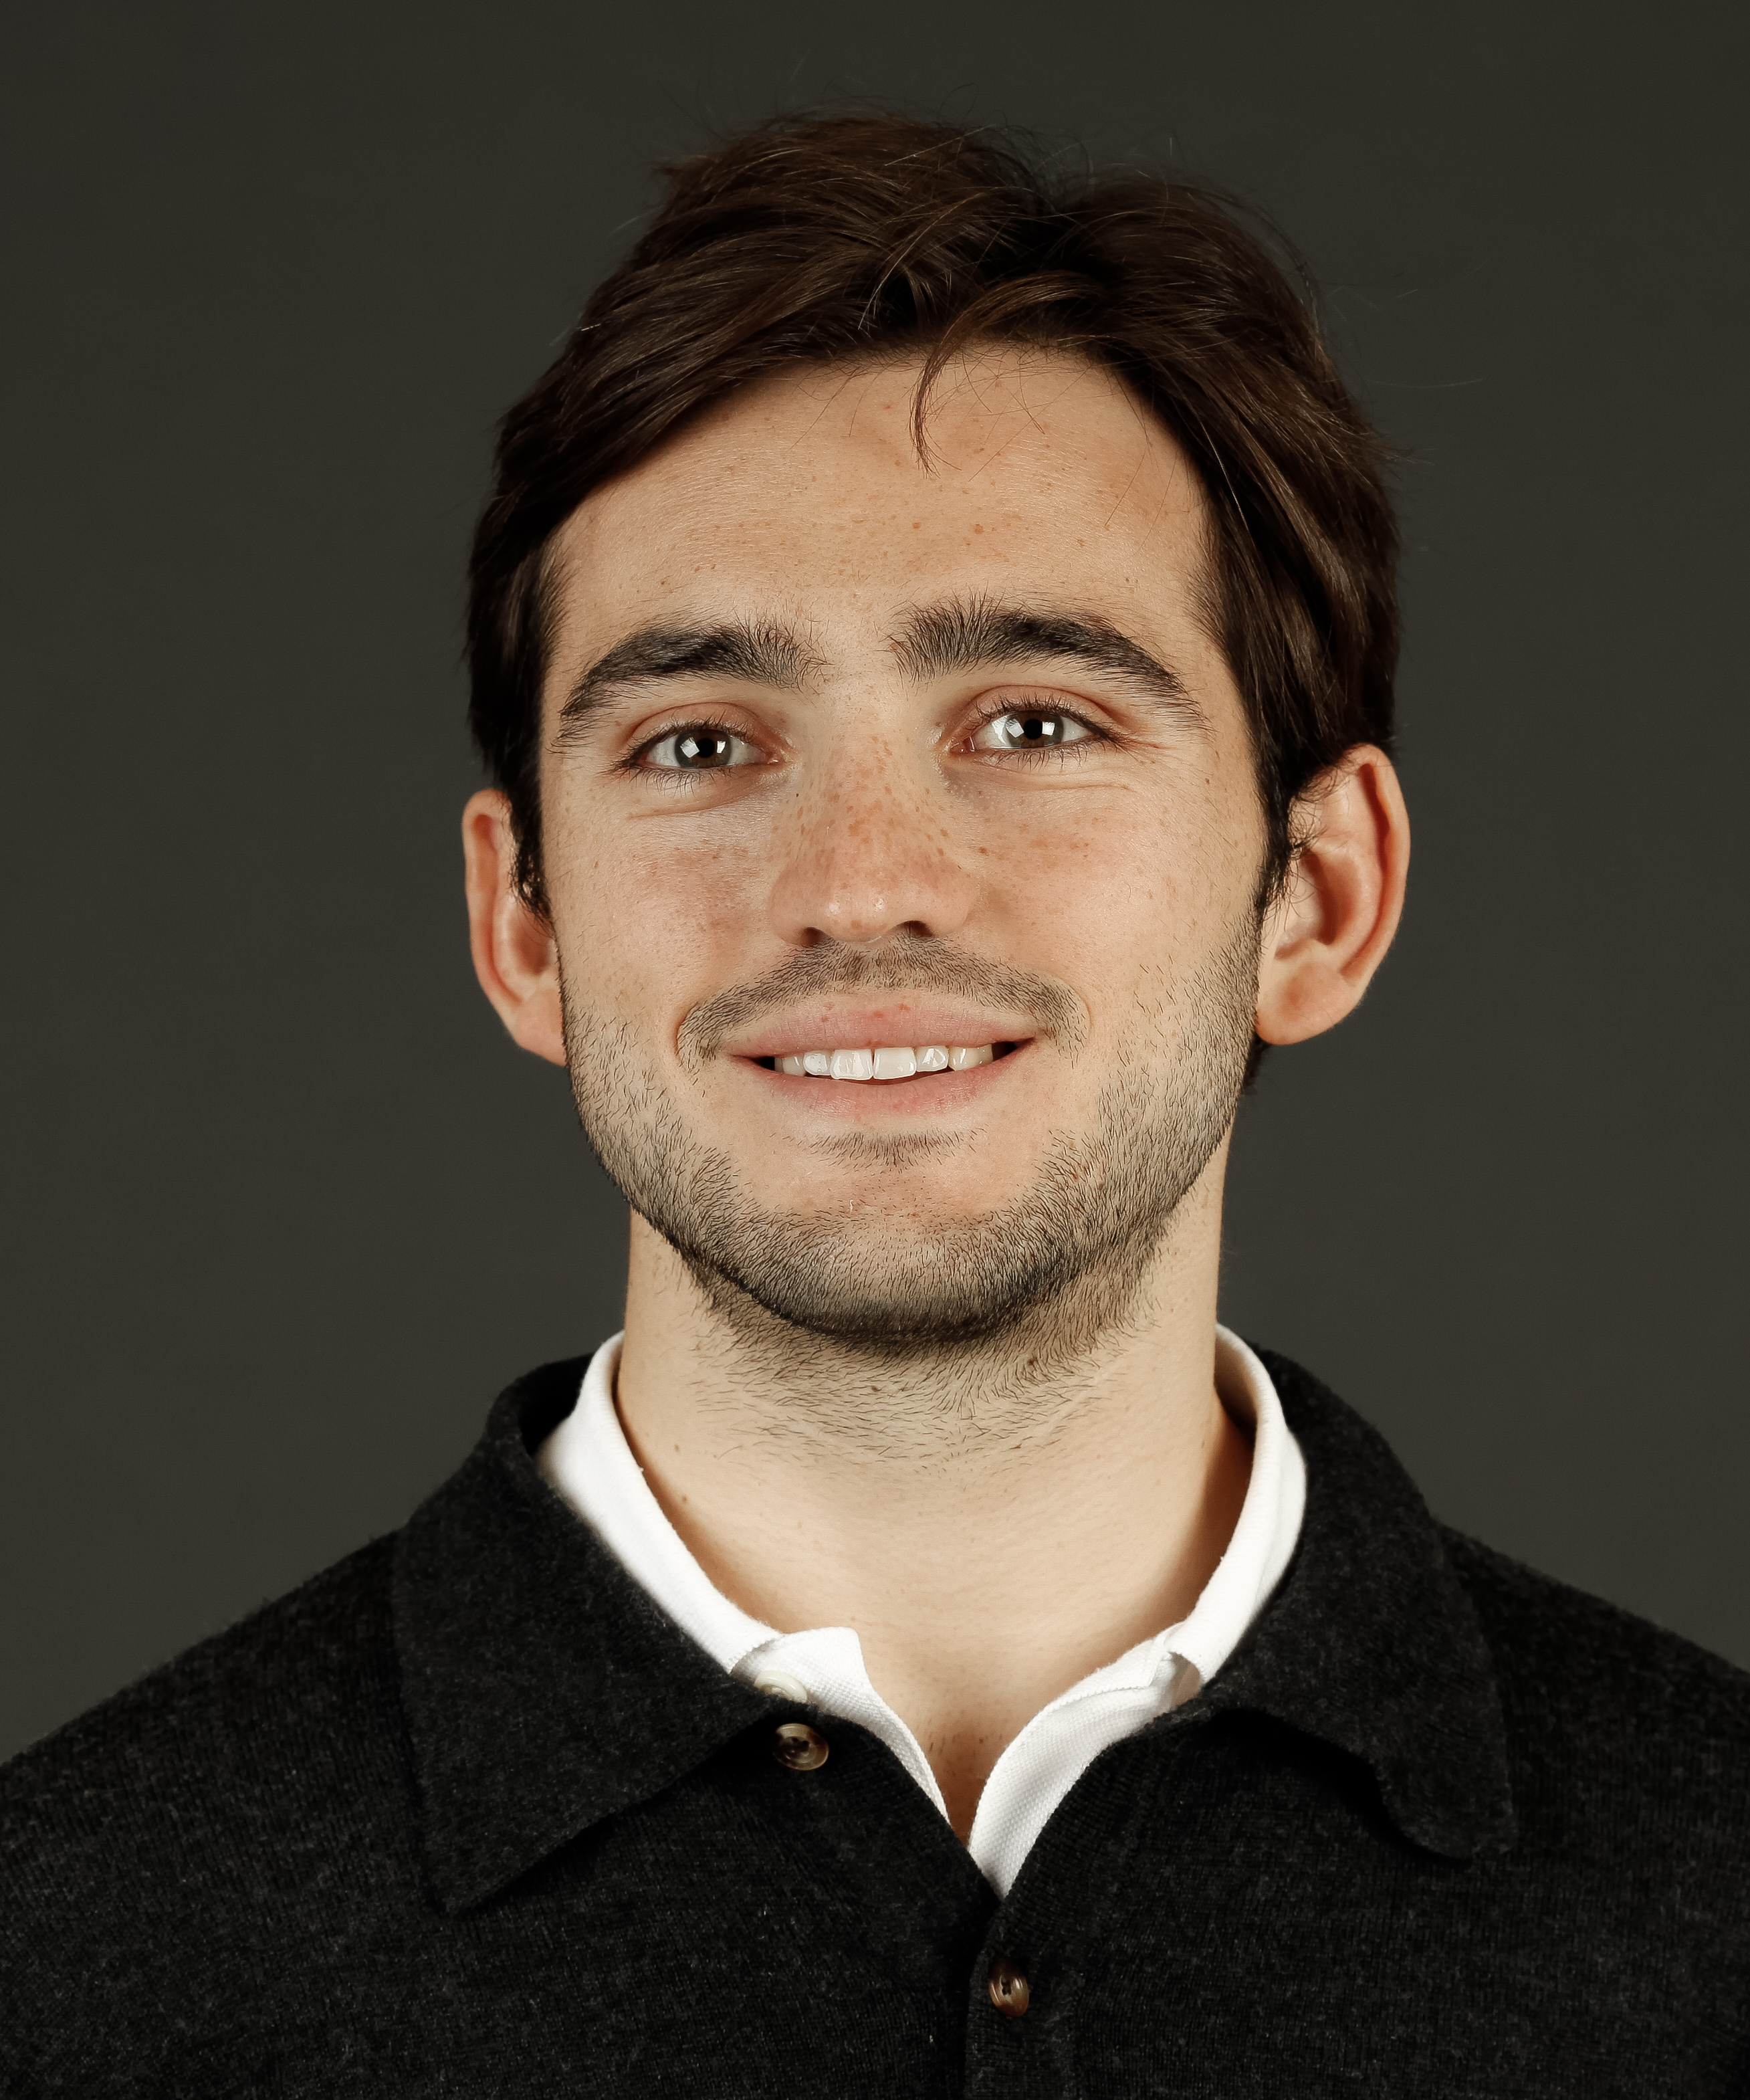
\includegraphics[width=2.1cm]{csem_img.jpg}}%
}%
\end{minipage} 
\end{table}

\section{Short Bio}
\begin{tabular}{p{\dimexpr1.5cm+\columnWidth}}
    I am a MSc student in advanced mathematics at the School of Mathematics from the Technical University of Catalonia, in Barcelona, Spain.
    I am focusing on graph theory, combinatorics and cryptography.
    Further, I also attend courses on distributed systems, concurrency, and networking from the Master in Research in Informatics.
    As a researcher, I collaborate with the Computer Architecture Department in my home university and with the Complex Systems Group of the Universit\'e de Neuch\^atel. 
    My main research interests are systems and security, with a strong mathematical foundation.
\end{tabular}

\section{Publications}
\begin{tabular}{p{\dimexpr1.5cm+\columnWidth}}
    C. Segarra, M. Lemay, R. Delgado-Gonzalo, and V. Schiavoni, \textbf{\textit{"Using Trusted Execution Environments for Secure Stream Processing of Medical Data"}}. DAIS'19, Copenhagen, Denmark, June 17-21, 2019. \\[3pt]
    C. Segarra, E. Muntan\'e, M. Lemay, V. Schiavoni, and  R. Delgado-Gonzalo, \textbf{\textit{"Secure Stream Processing for Medical Data"}}. IEEE EMBC'19, Berlin, Germany, July 23-27, 2019. \\
\end{tabular}

\section{Work Experience}
%
\begin{tabular}{R{1.5cm}|p{\columnWidth}}
    \emph{Current} & Research Collaborator at the \textbf{\textsc{Technical University of Catalonia - School of Informatics}} \\
    \textsc{10/2019} & \small{\emph{Computer Architecture Department} - Sup. Jordi Guitart, PhD }\\ 
    & \footnotesize{Year-long research collaboration with the Computer Architecture Department (DAC) of the School of Informatics (FIB) of the Technical University of Catalonia (UPC) in Barcelona, Spain. Under the supervision of Jordi Guitart, we work on live migration of distributed applications.}
\end{tabular}

\begin{tabular}{R{1.5cm}|p{\columnWidth}}
    \emph{Current} & Research Assistant at the \textbf{\textsc{Universit\'e de Neuch\^atel - Institut d'Informatique} (UniNe)} \\
    \textsc{08/2019} & \small{\emph{Complex Systems Group} - Sup. Valerio Schiavoni, PhD }\\ 
    & \footnotesize{Research collaborator with the Complex Systems Group from the UniNe. Currently working on an emulation platform for distributed applications. We simulate arbitrary topologies basing on the end-to-end properties of the links among the different nodes in the network, and dynamic link behaviours using traffic control functionalities available in the Linux Kernel.}
\end{tabular}

\begin{tabular}{R{1.5cm}|p{\columnWidth}}
    \textsc{07/2019} & Trainee at the \textbf{\textsc{Swiss Center for Electronics and Microtechnology} (CSEM)} \\
    \textsc{10/2018} & \small{\emph{Embedded Software Division} - Sup. Ricard Delgado Gonzalo, PhD }\\ 
    & \footnotesize{Intern at the Embedded Software Division of the CSEM in Neuch\^atel, CH, using Trusted Execution Environments to perform privacy-preserving computations on IoT medical devices. Developed a distributed streaming platform on Intel SGX and currently a secure implementation of the MQTT broker relying on TLS and ARM TrustZone. Collaborator in two H2020 EU Projects: ACTIVAGE and TABEDE. In the former, responsible of implementing part of the Security \& Privacy module and in the latter responsible of implementing the User Control Interface, visualizing data coming from a variety of IoT devices.}
\end{tabular}

\begin{tabular}{R{1.5cm}|p{\columnWidth}}
    \textsc{09/2018} & Trainee at \textbf{\textsc{Nokia Bell Labs}} \\
    \textsc{06/2018} & \small{\emph{Security Group} - Sup. Matteo Signorini, PhD and Matteo Pontecorvi, PhD}\\ 
& \footnotesize{Summer intern at the the Cybersecurity department at Nokia Bell Labs in Paris-Saclay, France. I developed a graph-based model to detect, cluster and classify chains of malicious transactions in the Bitcoin's Blockchain. By defining an abstraction layer atop the chain and an isomorphism class, we managed to identify a variety of malicious services.}
\end{tabular}

\begin{tabular}{R{1.5cm}|p{\columnWidth}}
    \textsc{06/2018} & Research Student at the \textbf{\textsc{Barcelona Supercomputing Center} (BSC)} \\
    \textsc{04/2017} & \small{\emph{Workflows and Distributed Computing Group} - Sup. Rosa M. Badia, PhD} \\ 
    & \footnotesize{Research student at the Workflows and Distributed Computing Group at the BSC in Barcelona, Spain. I developed, deployed and benchmarked a distributed implementation of the DBSCAN clustering algorithm using COMP Superscalar, a programming model for distributed computing. Evaluation was done in the \textit{Mare Nostrum} supercomputer.}
\end{tabular}

\section{Education}

\begin{tabular}{R{1.5cm}|p{\columnWidth}}	
    \textsc{07/2020} & Master in \textbf{\textsc{Advanced Mathematics and Mathematical Engineering} (MAMME)} \\ 
    \textsc{09/2019} & \small{\emph{Technical University of Catalonia}, UPC}\\
     & \footnotesize{MSc in Advanced Mathematics with a focus in Discrete Mathematics and Algorithms. Enrolled to courses from the Master in Research in Informatics (MIRI-UPC). Relevant courses cover: Graph Theory, Codes and Cryptography, and Concurrence, Parallelism, and Distributed Systems.}
\end{tabular}

\begin{tabular}{R{1.5cm}|p{\columnWidth}}	
    \textsc{05/2019} & Bachelor's degree in \textbf{\textsc{Mathematics}} \\ 
    \textsc{09/2014} & \small{\emph{Technical University of Catalonia}, UPC}\\
     & \footnotesize{BSc in Mathematics within a double degree program in the Interdisciplinary Higher Education Center (CFIS) at the UPC. Relevant coursework covers real and complex analysis, statistics, probability and graph theory, combinatorics and algorithms.}
\end{tabular}

\begin{tabular}{R{1.5cm}|p{\columnWidth}}	
    \textsc{05/2019} &  Bachelor`s degree in \textbf{\textsc{Telecommunications Science and Technology}}\\ 
    \textsc{09/2014} & \small{\emph{Technical University of Catalonia}, UPC} \\
     & \footnotesize{BSc in Telecommunications Engineering within a double degree program in the Interdisciplinary Higher Education Center (CFIS) at the UPC. Relevant coursework covers networking and concurrency, digital and analogical communications and real time digital signal processing.}
\end{tabular}

%\begin{tabular}{R{1.5cm}|p{13.8cm}}	
%    \textsc{05/2014} & Spanish Baccalaureate \\
%    \textsc{09/2013} & \small{\emph{Escola Betània-Patmos}, Barcelona} \\ 
%    &  Graduated with honors. \\
%\end{tabular}

%\section{Skills and Interests}

%\begin{tabular}{R{1.5cm}|p{13.8cm}}
%      %& \textbf{Distributed Systems} \\ %\textsc{DS}
%    & {My main background and interests comprise \textbf{distributed} and \textbf{decentralized} systems. I am also particularly interested in \textbf{networking}, \textbf{cryptography}, \textbf{security} and \textbf{data privacy}, specially in homomorphic encryption and trusted execution environments. Furthermore, \textbf{graph theory}, \textbf{combinatorics} and \textbf{probability} are math disciplines that I enjoy. In short, I am very interested in applying strong and founded mathematical concepts to distributed computing environments. On a lighter note, I read literature of all sorts and I train for and take part in amateur triathlons.}  \\
%\end{tabular}

%\begin{tabular}{R{1.5cm}|p{13.8cm}}
%      & \textbf{Security and Data Privacy} \\ %\textsc{BD}
%    & \footnotesize{The constant exposure we have to computers and the amount of data these process, makes ensuring security and privacy of vital importance. I am particularly interested in Trusted Execution Environments and Homomorphic Encryption for privacy-preserving computing techniques, and everything concerning data-at-rest and in-motion's security.}  \\
%\end{tabular}
%
%\begin{tabular}{R{1.5cm}|p{13.8cm}}
%      & \textbf{Graph Theory and Combinatorics} \\ %\textsc{GT \& C}
%    & \footnotesize{I am strongly interested in the areas of mathematics studying graphs, combinatorics and probability. I specially like the impact of these in distributed systems, coding theory and cryptography.}  \\
%\end{tabular}
%
%\begin{tabular}{R{1.5cm}|p{13.8cm}}
%      & \textbf{Other Interests} \\ %\textsc{OI}
%    & \footnotesize{On a lighter note, I also enjoy reading literature of all sorts. It allows me to maintain a global perspective whilst working on very particular topics. I train for and take part in amateur triathlons.}  \\
%\end{tabular}
\end{document}
